\documentclass[12pt, a4paper]{article}
% Preamble

% Load it during Section 1
\usepackage{setspace} % or \renewcommand{\baselinestretch}{1.5}
\onehalfspacing % or \doublespacing

% Load it during Graphic Section
\usepackage{graphicx}

% Load it during Math Section
\usepackage{amsmath}

% Load it during Reference Section
\usepackage[style = authoryear]{biblatex}
\addbibresource{reference.bib}

%\usepackage{fontspec} % Use XeTeX to compile
%\setmainfont[Ligatures=TeX]{Times New Roman} % EB Garamond

\title{Intro to \LaTeX{}}
\author{Brian Leung \\ University of Washington}
\date{\today}

\begin{document}

\maketitle

% \tableofcontents 
% \listoffigures
% \listoftables

\section{Line, Paragraph and Page Breaks}
Hello World! This is our first \LaTeX{} lesson. I really know nothing about it. But I'm very excite to learn about it. 
% An empty line starts a new paragraph

Hello World! This is our first \LaTeX{} lesson. I really know nothing about it. But I'm very excite to learn about it. \\ % Force a line break 
This is a new line. (But don't use \textbackslash \textbackslash{} to force a new paragraph.)

% Load \usepackage{setspace} and \onehalfspacing

%\newpage

\section{Basic Text Typesetting}

\subsection{Text formatting}
You can format words in many ways: 

This is \underline{important}. 

This is \textit{important}.

This is \textbf{important}.

This is super-duper \textbf{\textit{important}}.

I use \texttt{R} programming.

\textsc{This is special}.

\subsection{Special Characters and Symbols}
These symbols are reserved and need a backslash: \# \$ \% \^{} \& \_ \{ \} \~{} \textbackslash 

For quotation marks, you need to use two grave accent (under tilde) and two vertical quote: ``Please be careful.''

There are three types of dashes: -, --, --- 

Other common symbols include:  $\sim$ \slash \dots 

\subsection{Environments: Itemize, Enumerate, and Description}
\begin{itemize}
    \item First item
    \item Second item
        \begin{itemize}
        \item Sub-item
            \begin{itemize}
            \item Sub-sub-item
            \end{itemize}
        \end{itemize}
    \item Third item
\end{itemize}

\smallskip

\begin{enumerate}
    \item First lab
    \item Second lab
    \begin{enumerate}
        \item \LaTeX{} is really useful
    \end{enumerate}
\end{enumerate}

\section{Table}

\begin{table}[h]
    \begin{center}
        \begin{tabular}{l c r}
        Week & Date & Content \\
        \hline
        1  & Jan 10 & Intro to \texttt{R} \\
        2  & Jan 17 & Intro to \LaTeX{} \\
        3 & \multicolumn{2}{c}{\textit{No class this week}} \\
        4 & Jan 31 & Intro to \texttt{ggplot2} \\
        \end{tabular}
    \end{center}
\caption{Schedule of CSSS 569 labs}
\label{tab:schedule}
\end{table}

Please refer to Table \ref{tab:schedule} for the labs schedule on page \pageref{tab:schedule}.

\section{Graphics and Images}
% Load \usepackage{graphicx}
\begin{figure}[t]
    \centering
    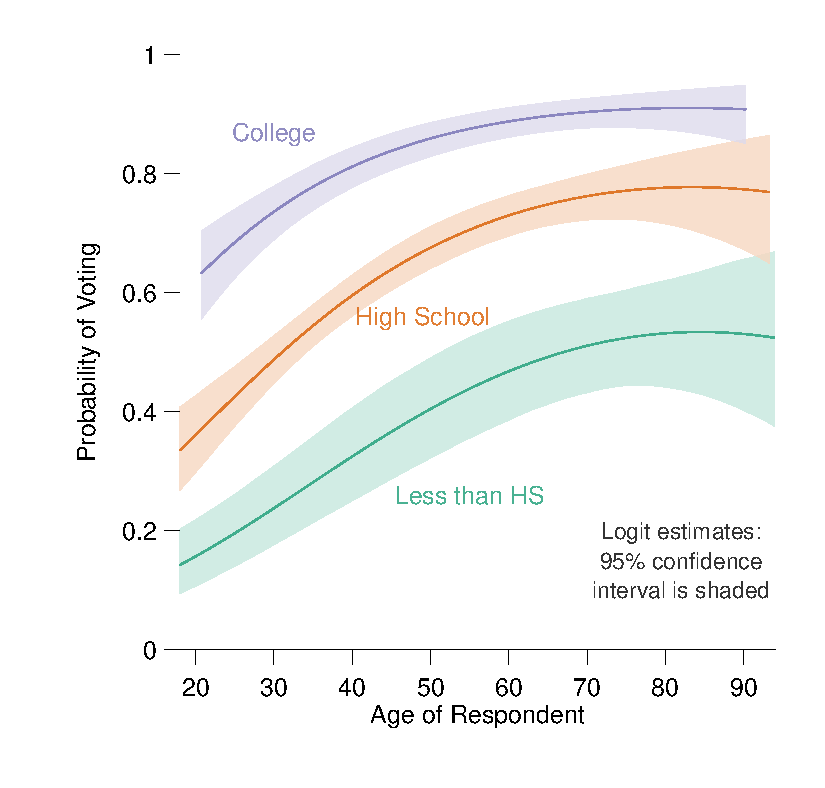
\includegraphics{figure/educationEV.pdf}
    \caption{Expected probability of voting conditional on education levels}
    \label{fig:edu}
\end{figure}

\section{Math formulas}
There are modes of writing maths in \LaTeX{}. 

The first mode is inline mode: $E = mc^2$ is an equation discovered by Einstein.

The second mode is display mode: Einstein proposes the following equation
\begin{equation}
E = mc^2
\end{equation}

Typesetting mathematics is easy in \LaTeX{}:
\begin{equation}
    e = \lim_{n \to \infty} \left( 1 + \frac{1}{n} \right)^n
\end{equation}

To split and align equations:
\begin{equation}
    \begin{split}
        f(x) & = (x + 5) \times (x - 7) \\
             & = x \cdot (x + 5)  - 7 \cdot (x + 5)  \\
             & = x^2 + 5x - 7x - 35 \\
             & = x^2 - 2x - 35
    \end{split}
\end{equation}

\section{Bibliography management}
Data visualization is fun \parencite{wilke_fundamentals_2019}. It is also beautiful \parencite{healy_data_2018}.

% \parencite and \textcite if style = authoryear

\printbibliography

% If have time: 
% 1) table of contents; list of figures and tables
% 2) go through changing font 
\end{document}